\documentclass[a4paper,12pt]{article}

\usepackage[english]{babel}

\usepackage[a4paper,top=2cm,bottom=2cm,left=3cm,right=3cm,marginparwidth=1.75cm]{geometry}

\usepackage{tabto}
\usepackage{amsmath}
\usepackage{graphicx}
\usepackage[colorlinks=true, allcolors=blue]{hyperref}
\usepackage{float}
\usepackage[T1]{fontenc}
\usepackage{frcursive}
\usepackage{calligra}
\usepackage{subcaption}
\newcommand{\setfont}[2]{{\fontfamily{#1}\selectfont #2}}


\title{Documentație: Offline Messenger}
\author{Leagăn Dan Adrian 2A5}
\date{Ianuarie 2022}

\begin{document}

\maketitle

\section {Introducere}

\tab
Proiectul Offline Messenger constă in crearea unei aplicații în care se pot loga mai mulți utilizatori, putând să trimită
mesaje unui alt utilizator. 

Funcționalitățile aplicației sunt vizualizarea comenzilor disponibile, crearea unui cont, logarea, vizualizarea listei cu utilizatorii înregistrați, trimiterea unui mesaj, vizualizarea conversației cu un anume utilizator, vizualizarea mesajelor necitite, raspunderea la un mesaj specific, delogarea și închiderea aplicației.
    
\section {Tehnologii utilizate}

\subsection{Modelul arhitecturii}

 \tab
 Realizarea conexiunii dintre server si client este constituită de modelul TCP/IP (Transmission Control Protocol / Internet Protocol).  Acest model permite conectarea a mai multor utilizatori simultan, servindu-i în mod concurent, verificând datele primite de către clienți, asigurând astfel protecție împotriva pierderii datelor.

\subsection{Alegerea modelului TCP în favoarea modelului UDP}
    
\tab
Am ales modelul TCP/IP deoarece informațiile trimise de client către server, și invers, trebuie să fie precise și să nu sufere modificări, acest model asigurând că datele nu sunt corupte sau pierdute în timpul trimiterii, verificând pachetele pentru erori.
    
\section {Arhitectura aplicatiei}

\subsection{Diagrama aplicației}

\begin{center}
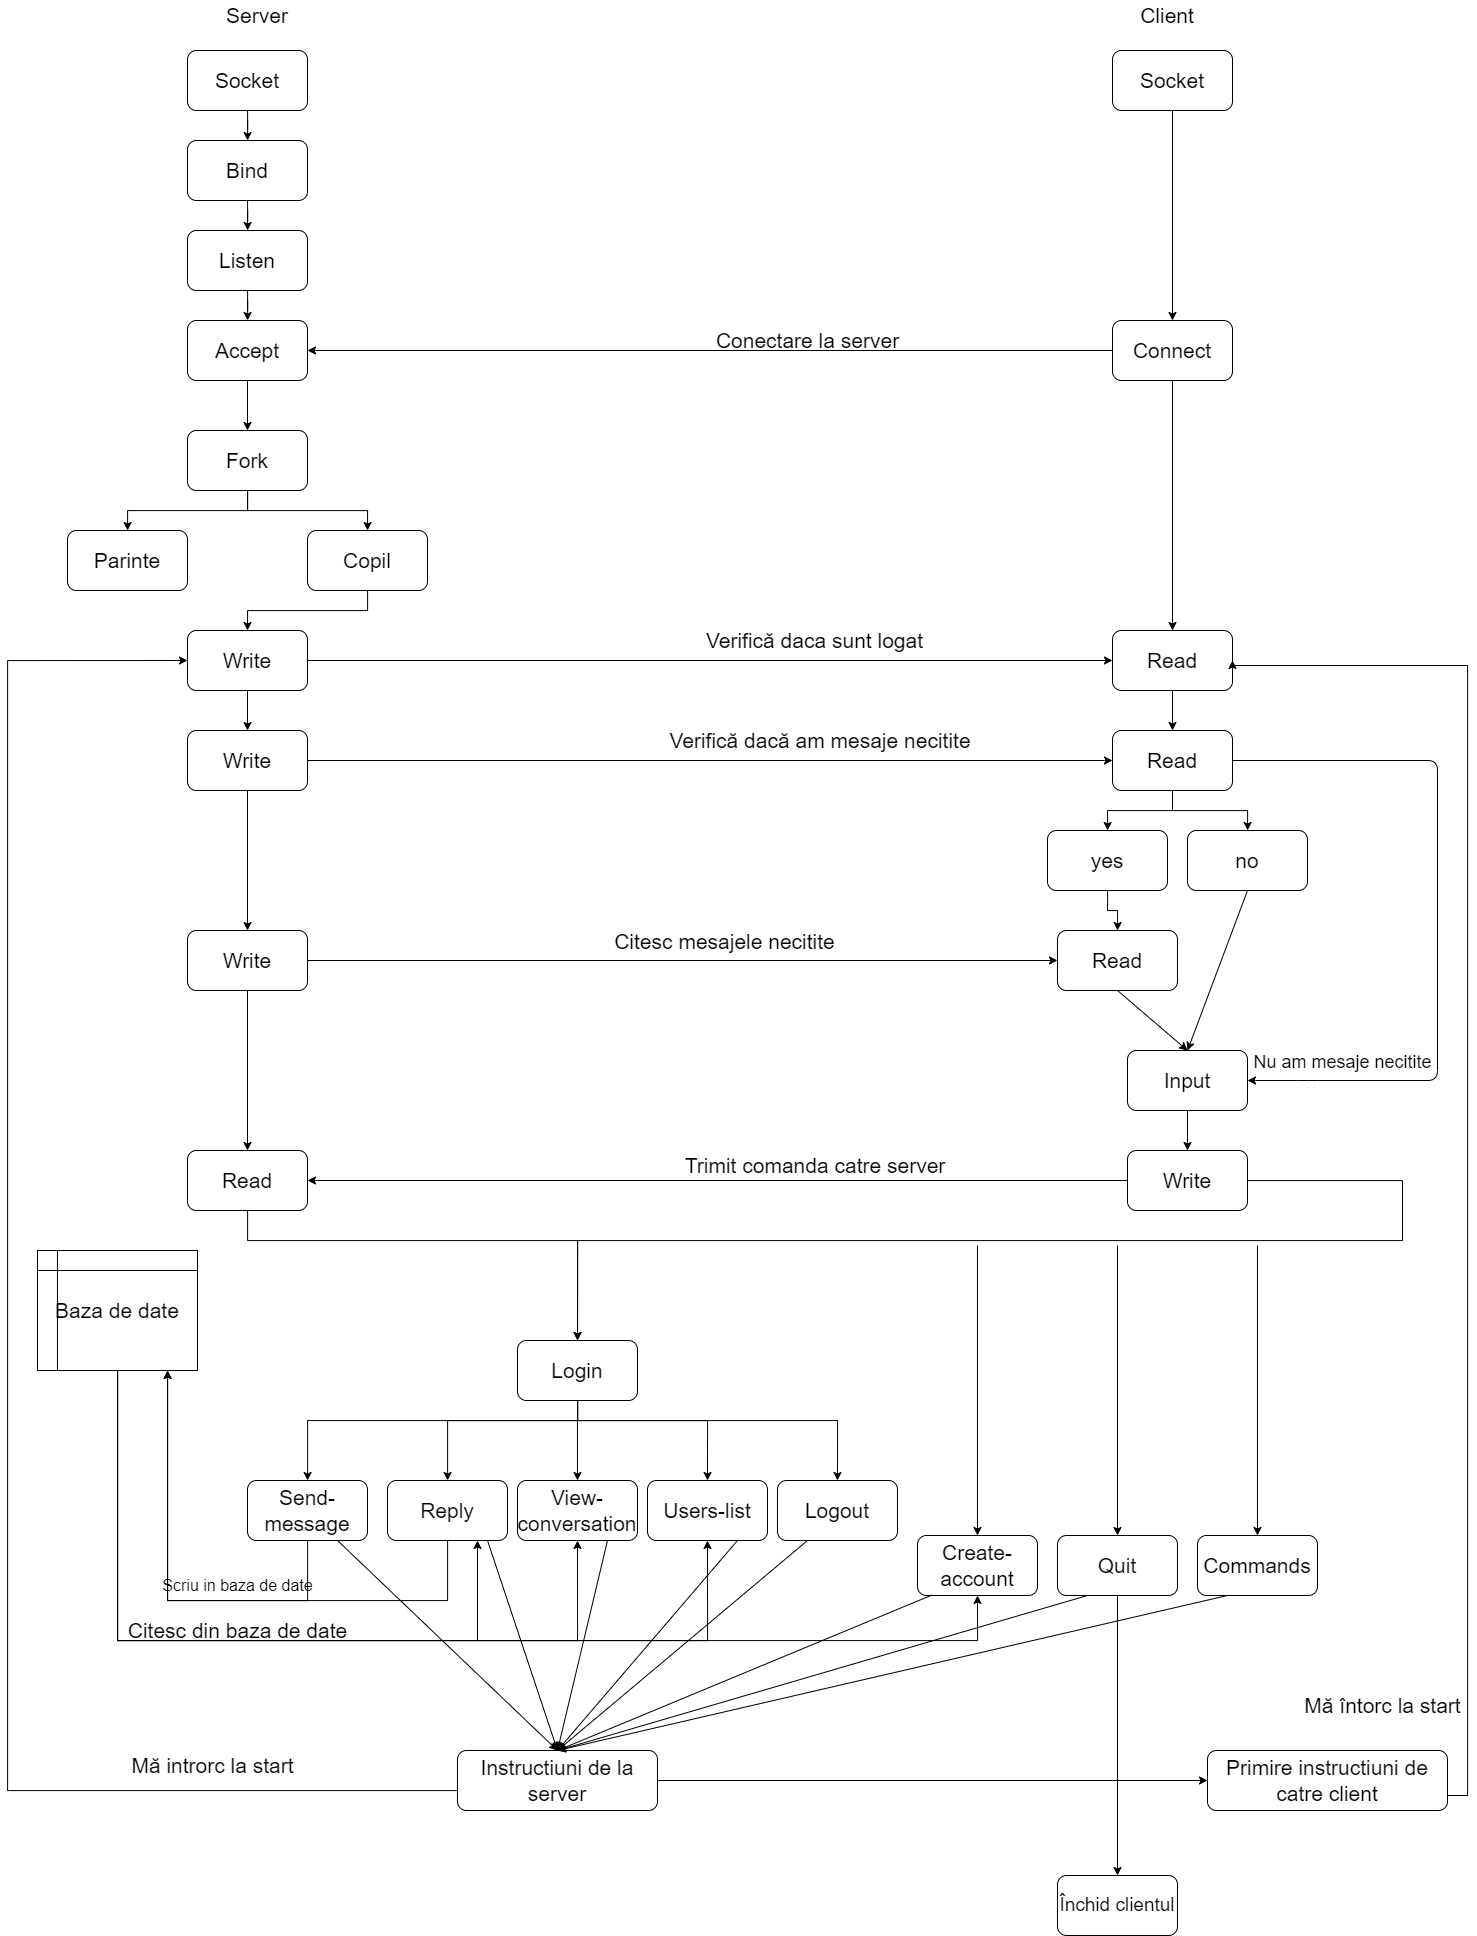
\includegraphics[width=1.1\textwidth]{Diagrama.png}
\end{center}

\subsection{Stocarea datelor}
\tab
Aplicația stochează datele intr-o bază de date, folosind sqlite3, instalat pe sistemul de operare. Aplicația deschide baza de date în timpul rulării, făcând modificări sau extrăgând date necesare pentru realizarea funcționalităților sale. 

Baza de date rămâne cu modificările făcute de aplicație, și după inchiderea acesteia, salvând conversațiile și conturile utilizatorilor până la următoarea accesare. Baza de date conține două tabele, "utilizatori", care conține username-urile și parolele utilizatorilor care și-au creat cont până in momentul respectiv, și "mesaje" care stochează mesajele utilizatorilor, destinatarul și expeditorul mesajului respectiv, statusul mesajului (dacă a fost văzut de către destinatar sau nu) și mesajul anterior pentru care s-a dat reply (dacă mesajul curent nu a fost dat ca reply, această coloana va avea în baza de date valoarea NULL).
    
\subsection{Conceptele aplicației}
 \tab
 După ce sunt deschise serverul și clientul, clientul așteaptă de la tastatură o comandă (ex: Login, Send-message). Unele comenzi sunt disponibile doar după ce a fost efectuată logarea (ex: Reply) iar altele sunt disponibile oricând (ex: Quit). După ce a fost introdusă comanda, clientul trimite această comandă la server, aceasta recunoscând-o și prelucrând corespunzător informațiile la care are acces prin baza de date. După prelucrare, trimite înapoi la client instrucțiuni, clientul afișând pe ecran în funcție de instrucțiunile primite.
    
    
\section {Detalii de implementare}

\subsection{Conectarea clientului}

\tab
După ce clientul se conectează la server, acestuia i se creează un proces copil care se va ocupa de client, urmând ca acesta să trimită înapoi datele cerute, sau sa modifice baza de date. Clientul primește de la tastatură o anumită comanda, pe care serverul o va recunoaște și va deschide apoi baza de date.
Dacă un al doilea client se conectează la server, în timp ce primul client incă este conectat, i se va crea un nou proces copil care va primi comenzile sale.

\subsection{Conectarea la baza de date}

\tab 
Pentru conectarea la baza de date sqlite3, s-au folosit următoarele funcții:

\bigskip

\begin{center}
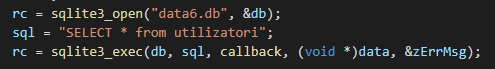
\includegraphics[width=0.7\textwidth]{baze_date.png}
\end{center}

\subsection{Comanda "Login"}

\tab
După ce a fost introdusă comanda "Login", aplicația va aștepta de la tastatură un nume de utilizator, după care se va conecta la server și va verifica în baza de date dacă există acest username. 
După acest pas, clientul va aștepta de la tastatura parola, și va verifica dacă aceasta corespunde numelui de utilizator introdus anterior.
Dacă aceasta corespunde, utilizatorul va fi logat în aplicație.

\bigskip

\begin{center}
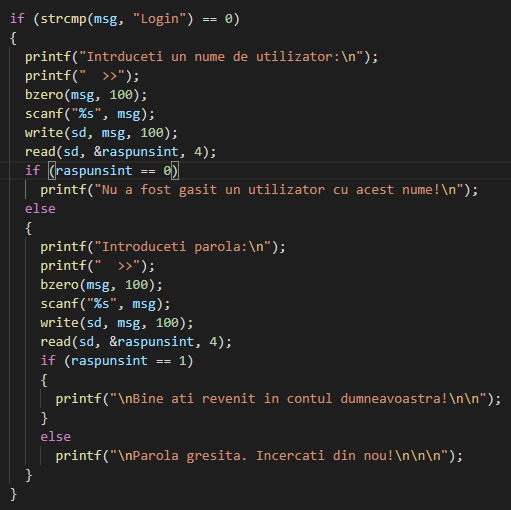
\includegraphics[width=0.7\textwidth]{Login.png}
\end{center}

\bigskip
\bigskip
\bigskip

\subsection{Comanda "Logout"}

\tab
La comanda "Logout", serverul va schimba variabila ce reține dacă clientul este logat, și va transmite o înștiințare către client.

\bigskip

\begin{center}
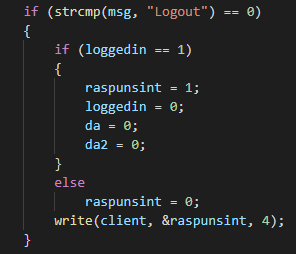
\includegraphics[width=0.5\textwidth]{Logout.png}
\end{center}

\subsection{Comanda "Users-list"}

\tab
Pentru fiecare comandă, serverul reține numele și parolele utilizatorilor într-o matrice de caractere (actualizând-o la fiecare comandă introdusă). La comanda "Users-list", acesta va forma un șir de caractere cu toți utilizatorii din matrice, trimițandu-l înapoi în client pentru afișare. 

\bigskip
\bigskip
\bigskip

\begin{center}
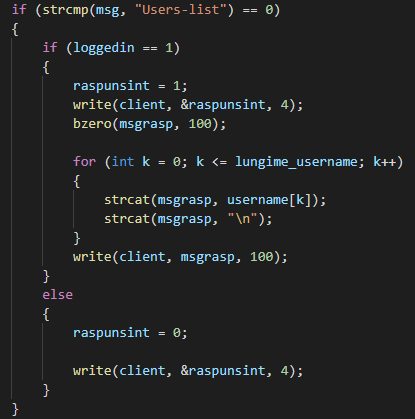
\includegraphics[width=0.5\textwidth]{Users-list.png}
\end{center}

\bigskip
\bigskip
\bigskip

\subsection{Comanda "Send-message"}

\tab
Comanda "Send-message" așteaptă de la tastatură numele unui utilizator căruia dorim să-i trimitem un mesaj. Clientul trimite numele către server, pentru verificare în baza de date. Dacă există un utilizator, clientul va aștepta mesajul, trimițandu-l în server, pentru a-l introduce în baza de date în tabelul "mesaje".

\bigskip
\bigskip
\bigskip

\begin{center}
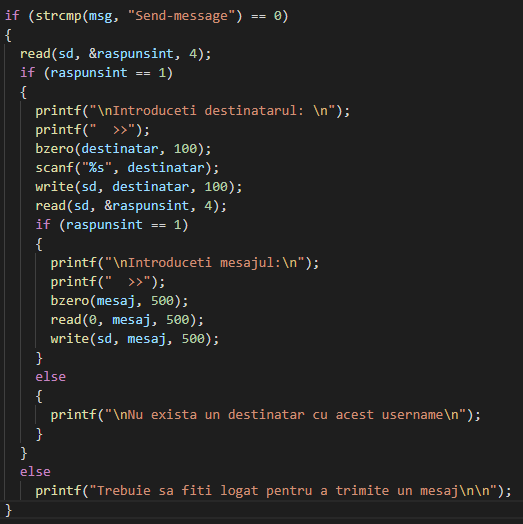
\includegraphics[width=0.7\textwidth]{Send-message.png}
\end{center}

\subsection{Comanda "Create-account"}

\tab
Aceasă comandă primește de la tastatura un username, și verifică baza de date pentru a nu exista un utilizator cu același nume. Dacă nu există, aplicația așteaptă o parolă, și apoi inserează în baza de date, trecând prima dată prin server, noul cont creat.

\bigskip

\begin{center}
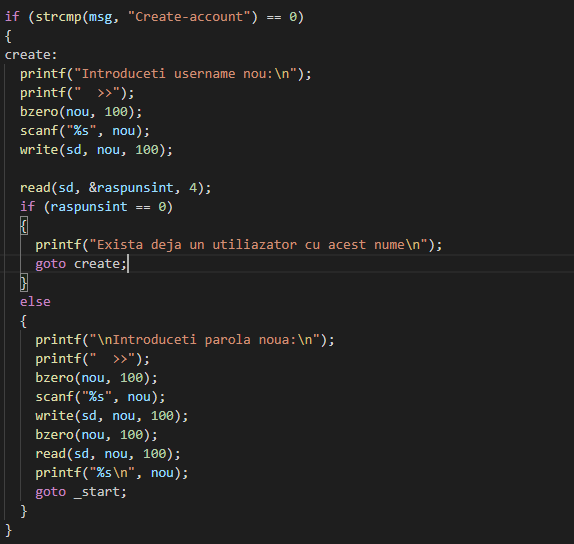
\includegraphics[width=0.5\textwidth]{Create-account.png}
\end{center}

\subsection{Comanda "View-conversation"}

\tab
La această comandă, serverul, după ce este contactat de client, deschide baza de date, și își formează/actualizează o matrice în care reține mesajele din baza de date, având grijă ca destinatarul și expeditorul să fie cei indicați de către client. După acest pas, trimite fiecare mesaj înapoi la client pentru afișare, și actualizează coloana "VĂZUT" în "1" pentru fiecare mesaj trimis și afișat.

\bigskip

\begin{center}
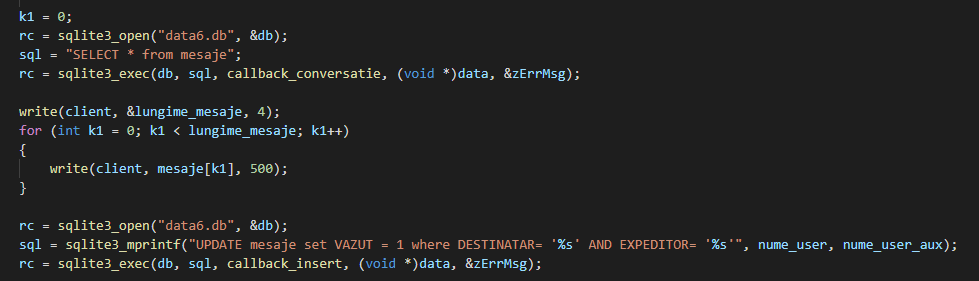
\includegraphics[width=0.8\textwidth]{View-conversation.png}
\end{center}

\subsection{Comanda "Reply"}

\tab
Codul de mai jos reprezintă momentul în care serverul a primit de la client mesajul pentru care se va da reply și mesajul cu care se va da reply. Serverul iși extrage destinatarul prin for, având apoi toate datele neccesare pentru a actualiza tabela mesaje cu noul mesaj.

\bigskip
\begin{center}
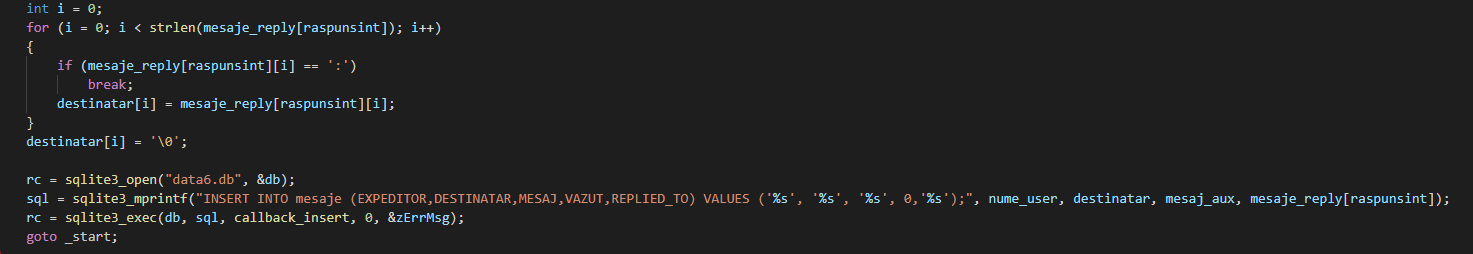
\includegraphics[width=1.0\textwidth]{Reply.png}
\end{center}

\subsection{Scenarii de utilizare}

\subsubsection {Scenariul 1: Utilizator nu are cont}

\tab
Dacă utilizatorul nu are cont, acesta poate să îșî creeze unul ("Create-account"), să vizualizeze comenzile aplicației ("Commands") sau să închidă aplicația ("Quit"). Va avea acces la comanda "Login", însă nu se va putea loga, și nu va avea acces la comenzile: Users-list, Send-message, Reply, View-conversation, Logout.

\subsubsection {Scenariul 2: Utilizatorul are cont}

\tab
Utilizatorul se poate loga în cont ("Login") pentru pentru a utiliza una din comenzile: Users-list, Send-message, Reply, View-conversation, Logout, sau poate folosi, fără a fi logat, comenzile: Create-account, Commands, Quit.

\subsubsection {Scenariul 3: Utilizatorul abia logat are mesaje necitite}

\tab
Utilizatorului îi va apărea o notificare despre faptul că are mesaje necitite, și va fi întrebat dacă dorește să le vizualizeze. Acesta poate introduce de la tastatură comanda "y" pentru vizualiza mesajele, sau "n" pentru a continua utilizarea aplicației.

\subsubsection {Scenariul 4: Utilizatorul abia logat nu are mesaje necitite}

\tab
Utilizatorul va fi informat cum că nu are mesaje necitite.

\subsubsection {Scenariul 5: Utilizatorul introduce o comandă necunoscută}

\tab
Va fi afișat pe ecran faptul că nu există o comandă precum cea introdusă.

\subsubsection {Scenariul 6: Utilizatorul introduce un username greșit la comenzile "Send-message", "View-conversation"}

\tab
Se va înștiința faptul că nu există un utilizator cu username-ul introdus.

\subsubsection {Scenariul 7: Utilizatorul delogat introduce comanda "Logout"}

\tab
Utilizatorul va fi informat că trebuie să fie logat într-un cont pentru a se putea deloga.

\section {Concluzii}

\tab
În concluzie, pentru a sumariza codul, clientul se conectează la server prin TCP/IP. După conectare, clientul primește o comandă de la tastatură și îl trimite serverului, această comandă fiind recunoscută atât de server cât și de client. Mesajele și utilizatorii sunt stocați într-o bază de date, unde se fac interogări și modificări în funcție de comandă. După ce comanda a fost efectuată, serverul se întoarce, așteptând o altă comandă de la client, iar clientul așteaptă o comandă introdusă de la tastatură.\newpage

Soluția ar putea fi îmbunătățită prin:\newline
-O interfață grafică destinată clientului care să-i permită deschiderea mai multor conversații simultan.\newline
-Posibilitatea de a șterge un mesaj trimis.\newline
-Posibilitatea de a modifica un mesaj trmis.\newline
-Posibilitatea unui utilizator de a-și șterge contul.\newline

\section {Bibliografie}

\begin{verbatim}
 https://www.tutorialspoint.com/sqlite/sqlite_c_cpp.htm
 
 https://www.razorsql.com/articles/sqlite_linux.html
 
 https://profs.info.uaic.ro/~computernetworks/cursullaboratorul.php
 
 https://profs.info.uaic.ro/~gcalancea/Laboratorul_7.pdf
 
 https://stackoverflow.com/questions/2942370
 
 https://www.sqlite.org/datatype3.html

 https://unix.stackexchange.com/questions/84813

 https://stackoverflow.com/questions/24194961
 
\end{verbatim}


\end{document}
